
\section{Vícios no treinamento}
\label{sec:sec-under-over-fitting}
\index{Overfitting}
\index{Underfitting}


Na área de pesquisa do ``aprendizado de máquina'' se estuda, entre outros muitos temas, 
como o erro no desempenho de um modelo ou sistema 
se relaciona com o método de treinamento e escolha das amostras.

Por exemplo, a Figura \ref{fig:fitting} mostra 3 casos que podem acontecer na 
etapa de treinamento de um modelo o qual procura realizar uma tarefa com o menor erro possível.
Estos casos podem ser: 
\begin{inparaitem}
\item sub-ajuste, 
\item ajuste adequado e 
\item sobre-ajuste.
\end{inparaitem}
\begin{figure}[!h]
  \centering
     \begin{subfigure}[b]{0.3\textwidth}
         \centering
         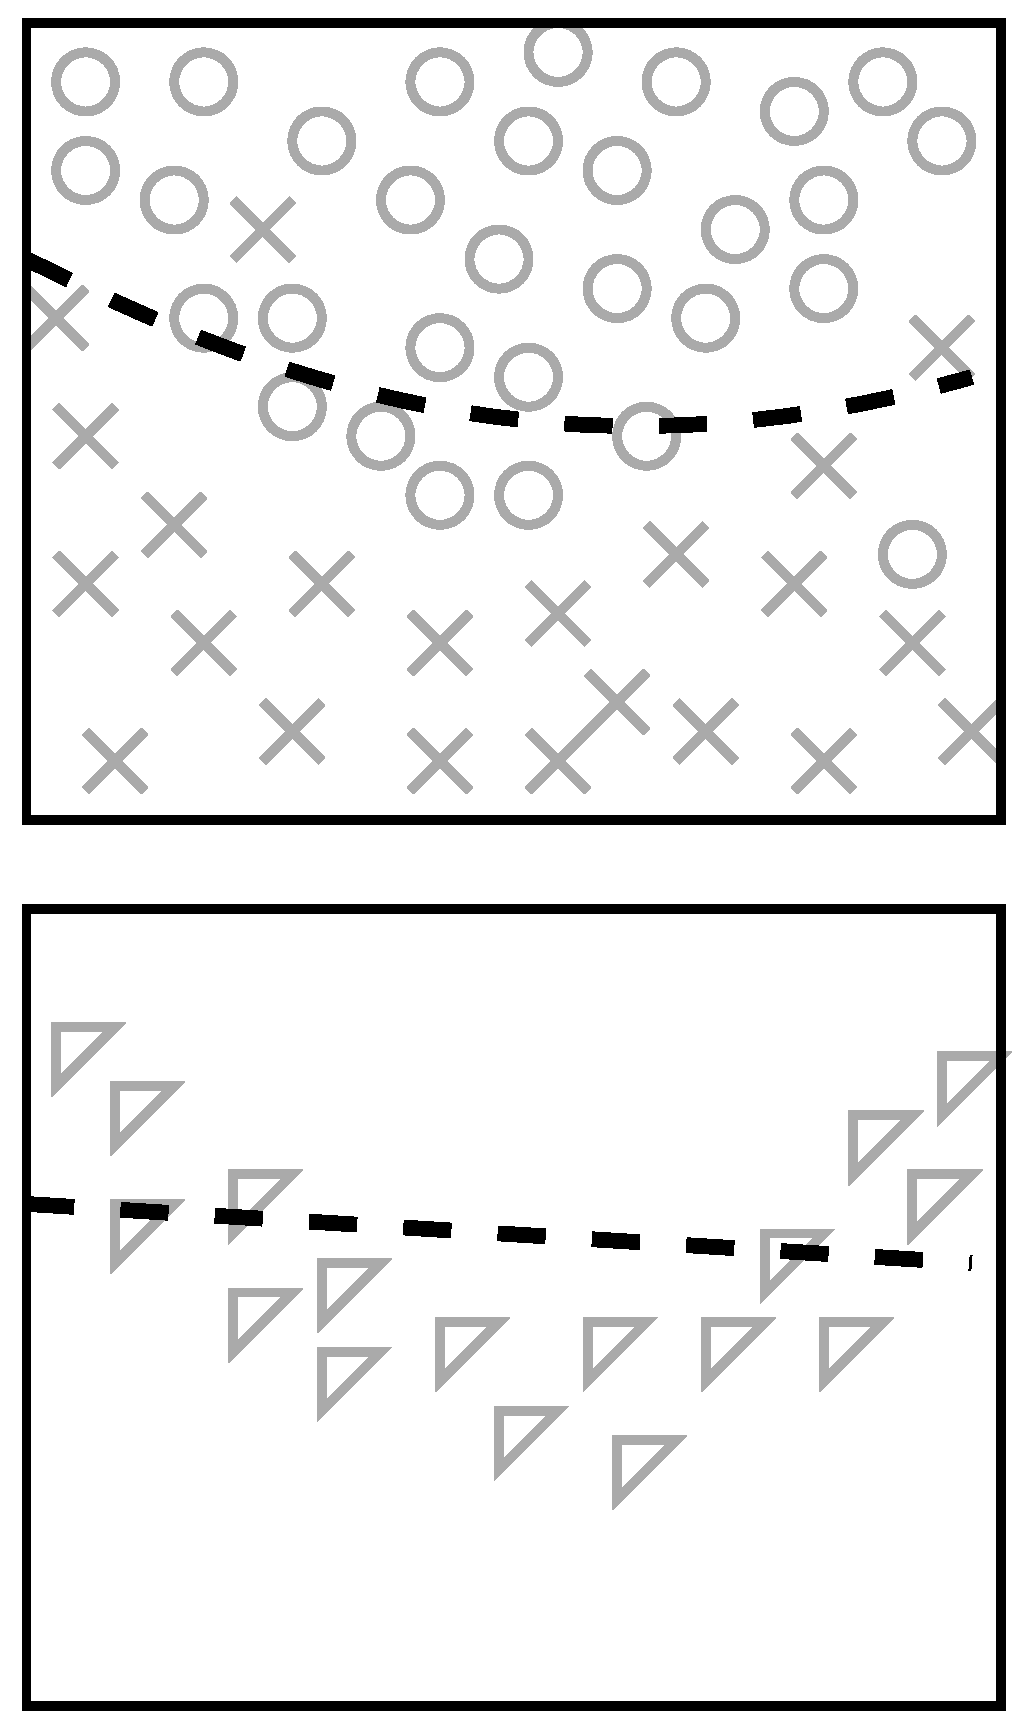
\includegraphics[width=0.8\textwidth]{chapters/cap-learning/fitting-under.eps} 
         \caption{Sub-ajustado ``underfitting''.}
         \label{fig:fitting:under}
     \end{subfigure}
     \quad
     \begin{subfigure}[b]{0.3\textwidth}
         \centering
         \includegraphics[width=0.8\textwidth]{chapters/cap-learning/fitting-robust.eps} 
         \caption{Ajuste adequado ou robusto.}
         \label{fig:fitting:robust}
     \end{subfigure}
     \quad
     \begin{subfigure}[b]{0.3\textwidth}
         \centering
         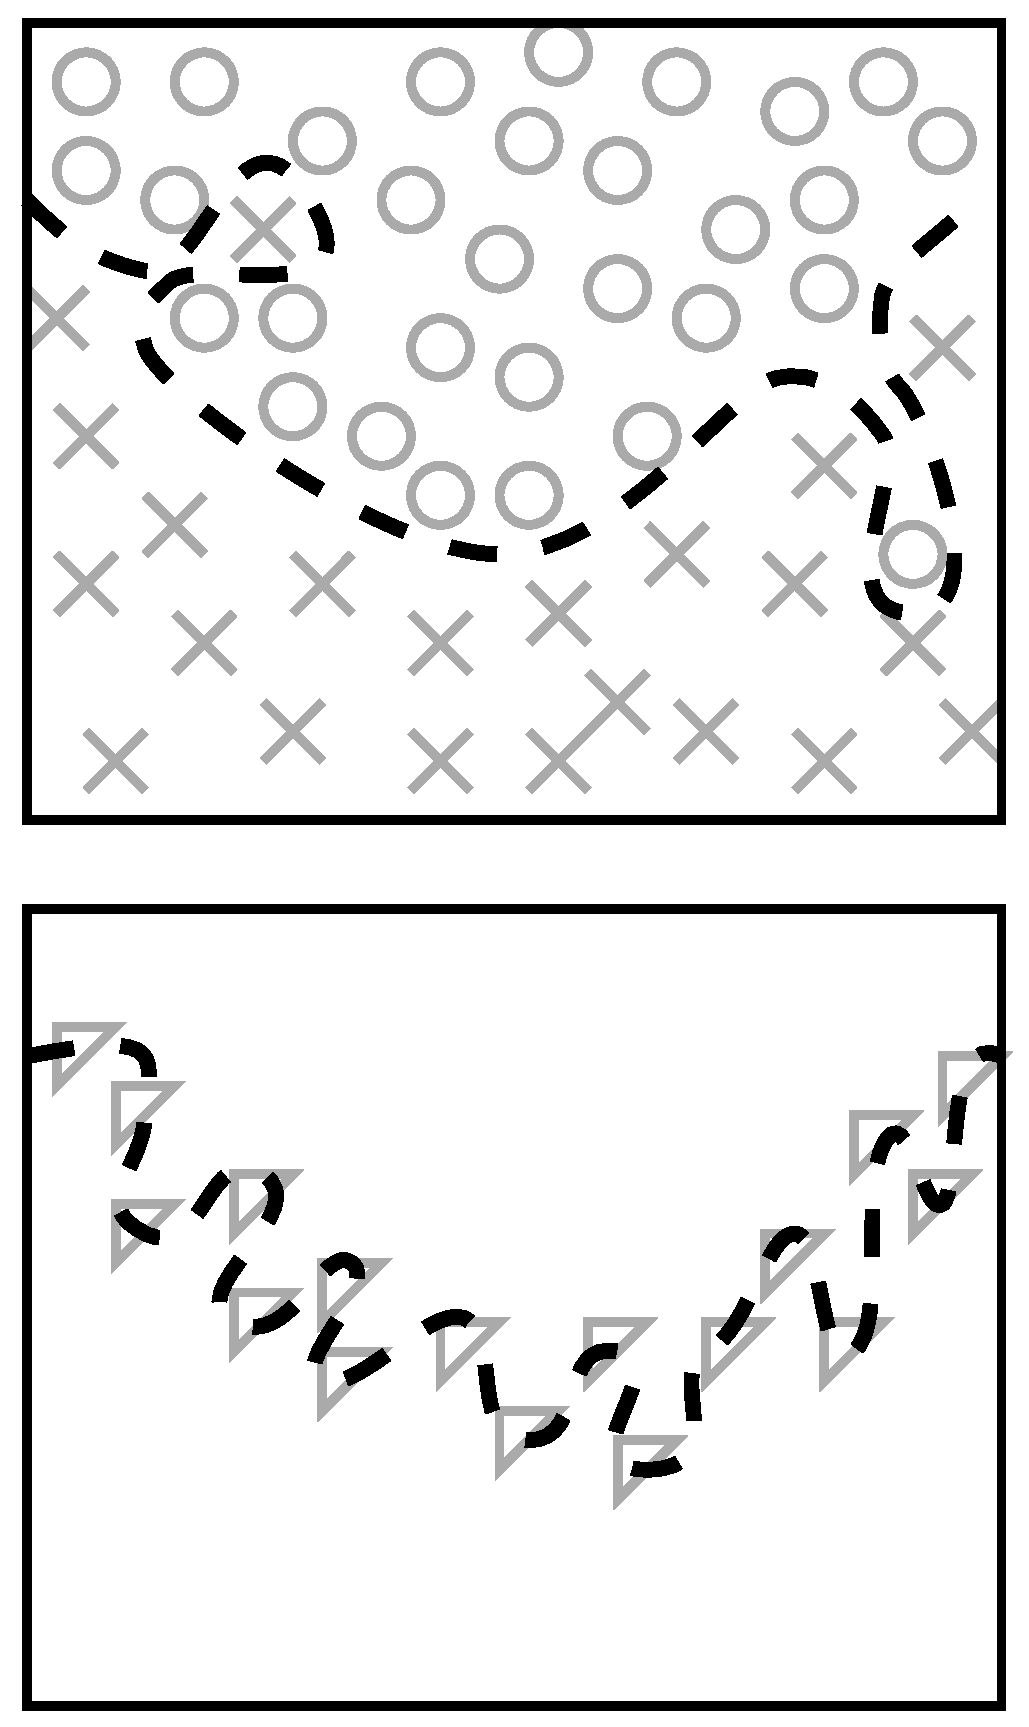
\includegraphics[width=0.8\textwidth]{chapters/cap-learning/fitting-over.eps} 
         \caption{Sobre-ajustado ``overfitting''.}
         \label{fig:fitting:over}
     \end{subfigure}
  \caption{Estados no processo de  aprendizagem.}
\label{fig:fitting}
\end{figure}

Na Figura \ref{fig:fitting:under} podemos ver um caso de subajuste, devido 
a que o modelo que usamos não é o adequado para descrever com pouco erro as relações 
nas amostras do treinamento. 
Também pode acontecer que tenham sido realizadas poucas épocas de treinamento 
e sejam necessárias mais iterações para melhorar o encaixe do modelo.  

A Figura \ref{fig:fitting:robust} mostra um ajuste adequado,
pois mesmo tendo erros de classificação, o modelo logra generalizar bem
as relações entre as amostras de treinamento; 
por outro lado, a boa generalização atribuída ao modelo
pode ser usada para converter este num detetor de quais amostras foram, na verdade, recebidas com erro.

A Figura \ref{fig:fitting:over} mostra um sobre ajuste,
pois o modelo perde toda capacidade de generalização ou predição do comportamento das amostras, 
o que provoca que mesmo tendo um erro de treinamento zero,
quando se introduz uma amostra de teste, o erro com esta tende a ser maior do esperado. 

Neste ponto podemos nos perguntar, como souber em qual destes 3 casos está nosso modelo
e como isto se relaciona com a dança?
Se extrapolamos este estudo a nosso processo de aprendizagem na dança,
perceberemos que em nosso caso o modelo/sistema é nosso conhecimento junto com nosso corpo em movimento na dança,
as épocas correspondem a nosso tempo de treinamento, e as amostras
são, por exemplo, as dinâmicas usadas, os pares de dança ou em geral cada contexto no qual medimos nosso desempenho.  

Assim quando realizamos um treinamento debemos estar conscientes y alertas 
de analisar se estamos com um subajuste, um sobreajuste ou um ajuste adequado.
\begin{example}[Treinando com nosso par de dança]
\label{ex:fitting:1}
Se realizamos treinamentos de forma continua e exclusiva com um único par de dança,
nos perceberemos que
com o aumento das épocas de treinamento chega a acontecer uma grande diminuição do erro
de nosso desempenho na dança com essa pessoa. Nesse contexto podemos estar em 3 casos:
\begin{itemize}
\item \textbf{Subajuste:} O erro do desempenho não é o suficientemente baixo, este ainda pode 
melhorar com mais tempo de treinamento do par.
\item \textbf{Ajuste adequado:} O erro existe e é baixo, 
se consegue generalizar mantendo o mesmo desempenho para outras dinâmicas de trabalho não conhecidas, 
inclusive com outro par de dança. 
\item \textbf{Sobreajuste:} O erro da performance do par é extremadamente baixo, 
o par tem uma coordenação perfeita para uma dinâmica de treinamento, porém
 ante uma mínima mudança do âmbito ou de par de dança, 
 o erro de desempenho aumenta de forma considerável.
\end{itemize}
\end{example}

\subsection{Como identificar?}
Uma forma de identificar se estamos num caso de subajuste, sobreajuste ou um ajuste adequado,
é usando curvas de aprendizagem como a mostrada na Figura \ref{fig:fitting:curve}.
\begin{figure}[!h]
  \centering
    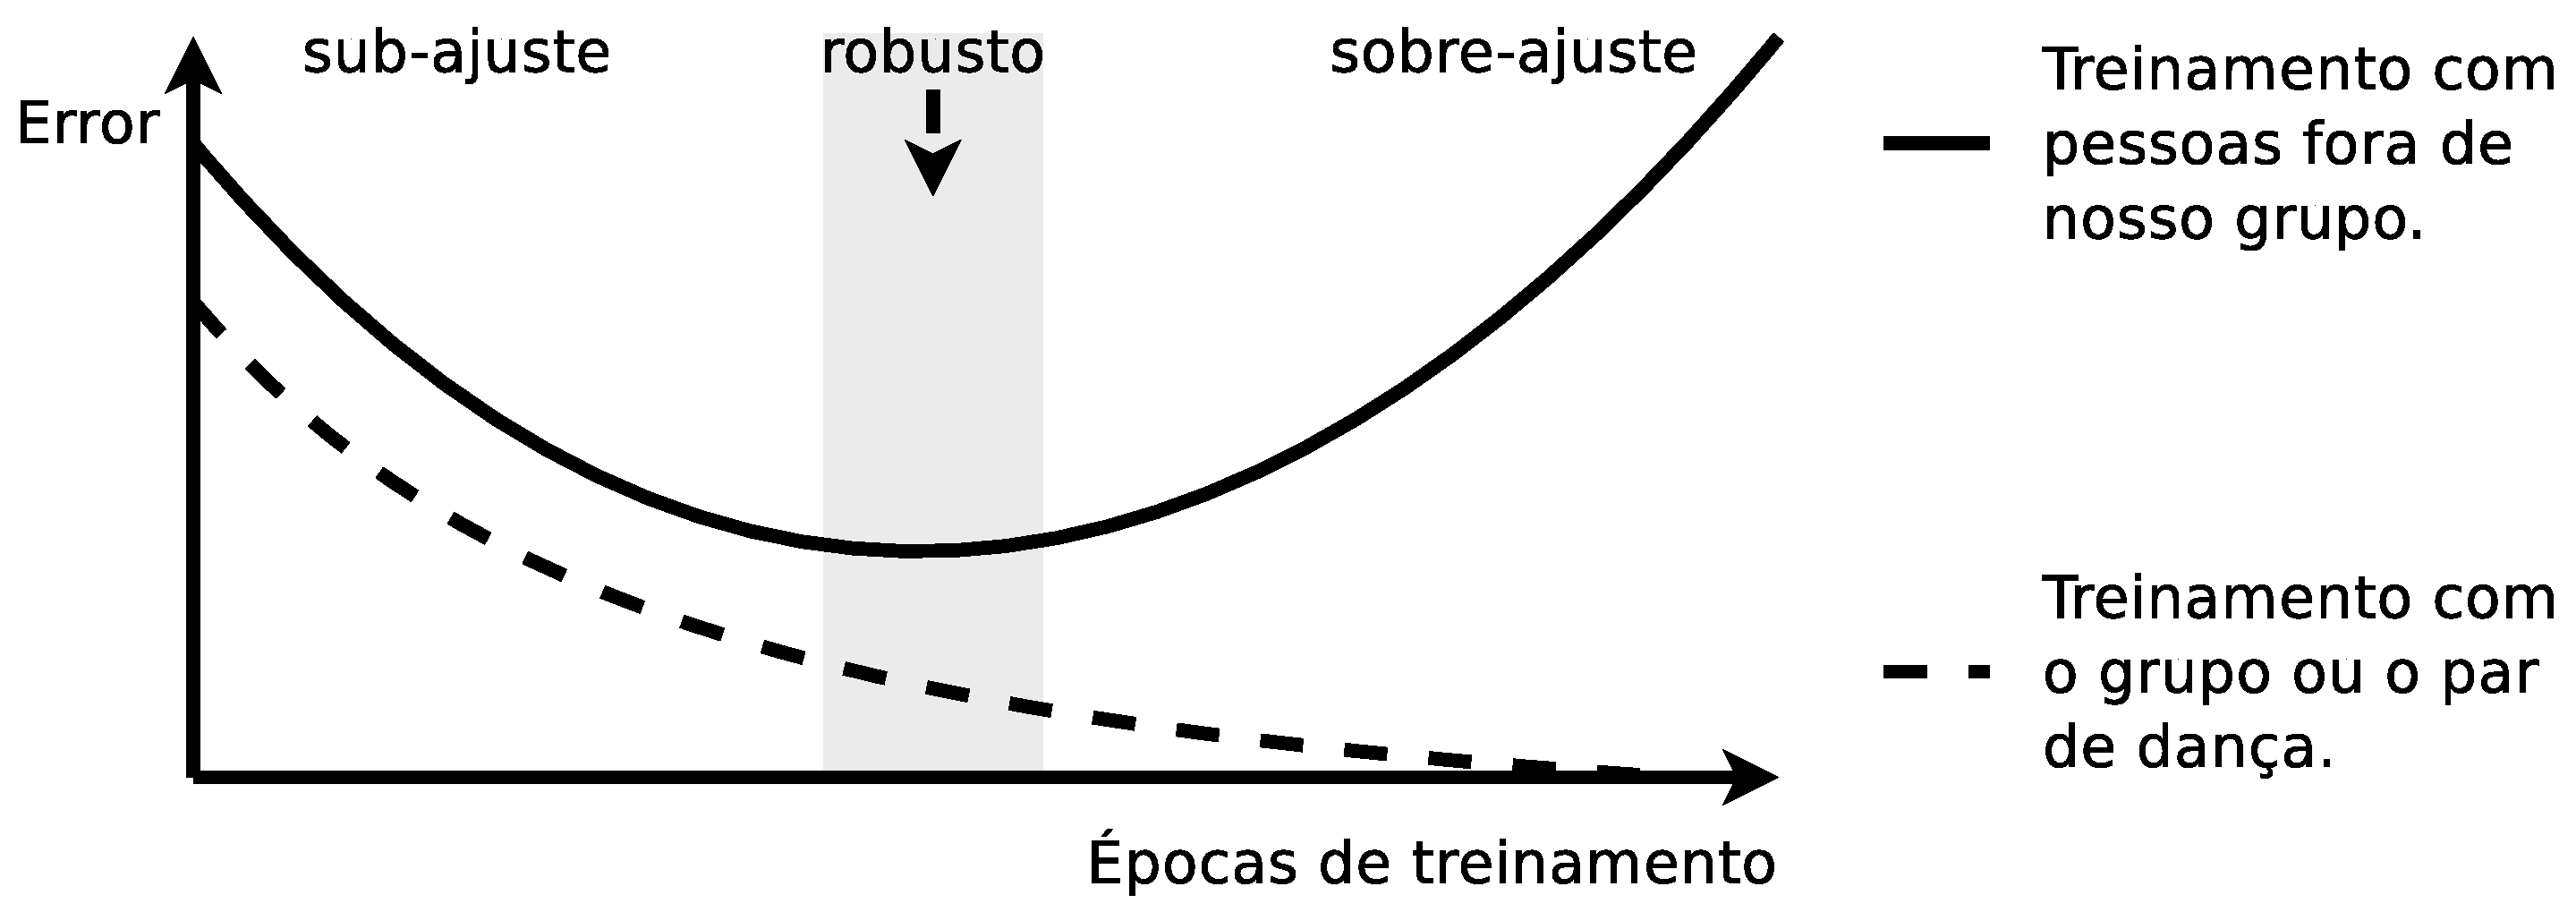
\includegraphics[width=0.7\textwidth]{chapters/cap-learning/fitting-error.eps} 
  \caption{Erro no aprendizagem vs. as épocas (repetições) no treinamento.}
\label{fig:fitting:curve}
\end{figure}
Esta figura descreve o error na nossa performance na dança
em relação à quantidade de nossas épocas de treinamento.
A primeira curva (linha pontuada) representa como o erro no nosso desempenho diminui
monotonicamente com o aumento das épocas de nosso treinamento com, por exemplo, nosso par de dança ou
nosso grupo de dança.
Por outro lado a segunda curva (linha sólida) mostra que o erro de no nosso desempenho
diminui até um tempo determinado e logo o erro cresce.
Esse momento, onde nosso erro é mínimo, é o momento adequado para deter 
as mudanças que realizamos sobre nós mesmos no nosso processo de treinamento/aprendizado 
com um âmbito e técnica especifica, é dizer é o momento de mudar de estrategia de aprendizado, de objetivo ou de contexto.  

O problema da segunda curva acontece devido a que num ponto determinado perdemos 
nosso poder de generalização e iniciamos a decorar detalhes específicos, de nosso 
par de dança, grupo de trabalho, sequencia do movimento ou da música.
\begin{comment}
\begin{example}[Treinando com sobreajuste]
Pode ser dar o caso que cada um do par de dança tenha decorado as manias do outro,
e ambos não estejam realizando algumas ações pois o par cobre esses erros, pelo que 
ao dançar com outras pessoas estas faltas se evidenciam.
\end{example}
\end{comment}

Assim, uma forma de solucionar este problema é ter um grupo de treinamento e 
um grupo de teste, de modo que em todo momento conferimos que o aprendido 
é generalizável para outras pessoas e contextos fora de nosso âmbito de trabalho.


